\documentclass{article}
\usepackage{mathtools,amssymb}
\usepackage{float,graphicx}
\usepackage{nopageno}
\usepackage[letterpaper]{geometry}

\setlength{\parindent}{0in}


\begin{document}

\begin{enumerate}
\item \underline{\hspace{3in}} (common fraction)\vspace{1cm}
\item \underline{\hspace{3in}}\vspace{1cm}
\item \underline{\hspace{3in}} (in terms of $\pi$)\vspace{1cm}
\item \underline{\hspace{3in}} (in terms of $\pi$)\vspace{1cm}
\item \underline{\hspace{3in}} (in terms of $\pi$)\vspace{1cm}
\item \underline{\hspace{3in}} (in terms of $\pi$)\vspace{1cm}
\item \underline{\hspace{3in}} (simplest radical form)\vspace{1cm}
\item \underline{\hspace{3in}} (in terms of $\pi$, simplest radical form)\vspace{1cm}
\item Each face of a uniform hexagonal prism is to be colored red or blue. In how many ways can this be done if two colorings are considered equivalent whenever one can be rotated to get the other? (A polyhedron is \emph{uniform} if all of its faces are regular polygons.)
\vspace{1cm}
\item In the figure below, lines $\overline{CD}$ and $\overline{EF}$ are tangent to both circles $A$ and $B$. If the radii of the circles are integers, $CD = 12$, and $EF = 10$, then what is $AB$? Express your answer in simplest radical form.
\begin{center}
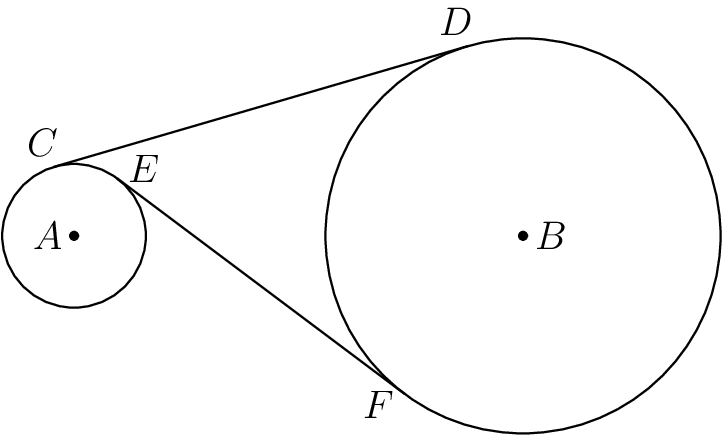
\includegraphics[scale=0.2]{circles.png}
\end{center}
\end{enumerate}


\newpage

\begin{enumerate}
\item $2/3$ (\emph{MATHCOUNTS 2013: School Sprint})\vspace{1cm}
\item $16$ (\emph{MATHCOUNTS 2008: School Team})\vspace{1cm}
\item $26 + 17\pi$ (\emph{MATHCOUNTS 2013: State Countdown})\vspace{1cm}
\item $\pi$\vspace{1cm}
\item $8\pi - 8$ (\emph{MATHCOUNTS 1994: School Team})\vspace{1cm}
\item $8\pi - 16$ (\emph{MATHCOUNTS 1991: National Countdown})\vspace{1cm}
\item $192 + 128\sqrt{3}$\vspace{1cm}
\item $36 - 12\sqrt{3} - 4\pi$ (\emph{MATHCOUNTS 1991: National Team})\vspace{1cm}
\item Each face of a uniform hexagonal prism is to be colored red or blue. In how many ways can this be done if two colorings are considered equivalent whenever one can be rotated to get the other? (A polyhedron is \emph{uniform} if all of its faces are regular polygons.) $\boxed{40}$
\vspace{1cm}
\item In the figure below, lines $\overline{CD}$ and $\overline{EF}$ are tangent to both circles $A$ and $B$. If the radii of the circles are integers, $CD = 12$, and $EF = 10$, then what is $AB$? Express your answer in simplest radical form. $\boxed{2\sqrt{61}}$
\begin{center}
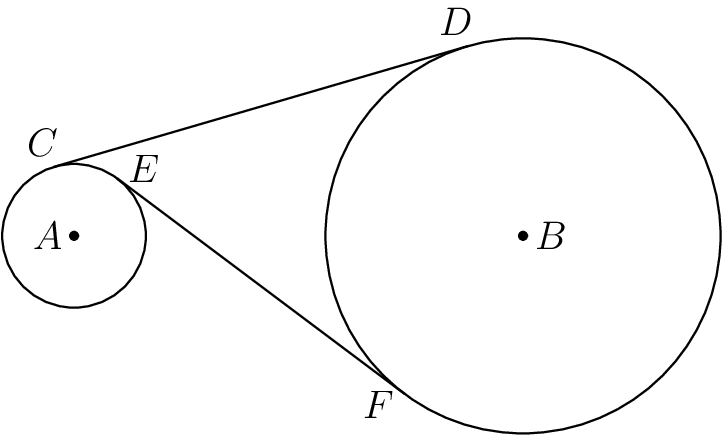
\includegraphics[scale=0.18]{circles.png}
\end{center}
\end{enumerate}

\end{document}

